\chapter{Existence and Absence of Hopf Bifurcation in Phosphorylation-Dephosphorylation CRN}

\section{What even \textbf{is} a bifurcation?}
To better generalize them, it'd be best to also define the notion of:

\begin{definition}
	\textbf{Invariant sets}.

	Taking the Auton. sys.
	\begin{equation}\label{invar_set_auton_sys}
		\dot{y} = f(y) , y(0) = y_0, y \in \mathbb{R}^n
	\end{equation}

	A state-set $S \subseteq \mathbb{R}^n$ of \ref{invar_set_auton_sys} is \textbf{invariant} if $\forall y_0 \in S, \forall t \geq 0: y(t) \in S$
\end{definition}

As you can see by this above definition, equilibria are also particular cases of invariant sets, themselves.

They also fall into stability classes that can be defined as in Def. \ref{equilibrium_stability}, but replacing
\[
	"y_0" \text{ with } "S \subseteq \mathbb{R}^n \text{ }"
\]
and
\[
	" \dotso \norm{y(t) - y_0} \dotso" \text{ with } "\dotso \text{ inf}\{ \norm{y(t) - s} : s \in S  \} \dotso \text{ }"
\]
The Jacobian (linearization), generally, would also not be as useful in this context anymore.
\newpage
Now consider we have a system as above, except it now depends on an extra parameter $\mu$, which remains constant \textbf{during} our "experiment".
\begin{equation}\label{auton_parameter_sys_compact}
	\dot{y} = f_\mu(y).
\end{equation}

This could be, for example, the length of the pendulum $L$, in \ref{damped_pendulum}, or its damping coefficient $c$. Honestly generalizing it even more, it could even be the gravitational constant $g$. Hence, this parameter can, of course be a \textbf{vector} of such parameters.

The way the parameter $\mu$ varies also induces variations in the topology and dynamics of the system. That's obvious since this is kind of the point of parameters in systems.

What can vary though can be trivial or more interesting.

The positions of invariant sets, for example can vary continuously

during changes in $\mu$; that's usually normal.

But what's more interesting is when these change their \textbf{stability} altogether, equilibria disappear completely / appear out of thin-air - or, even - collide with other invariant sets.

This odd behavior is called a \textbf{bifurcation}, and $\mu$, in this case is a \textbf{bifurcation parameter}.

The former types of bifurcations I talked about previously are called \textbf{local}, those in which changes in stability can only be considered mostly for \textbf{isolated equilibria}, individually, or other invariant sets whose stability can be analyzed \textbf{locally}, via the system's linearization at a point.

The latter are \textbf{global}, which are more complex and require greater understanding of the system beyond a local linearization, but that falls into the special-case category described in the last paragraphs of the previous chapter, and so far all I know about Mr. Prof. Lyapunov as of now is that his brother was pianist. But thankfully our interest for this work lies with local bifurcations, so we'll be ignoring this for now, maybe I'll come back to it during my Master's (not).

To better define and illustrate them for the 1-D case and give example of bifurcations for such dimension, we could instead write our vector field $f$ as depending on $\mu$ in addition to the unknown function $y$.
\begin{equation}\label{eq:1-d_bif_sys}
	\dot{y} = f(y, \mu).
\end{equation}
And assume $f \in C^k(\mathbb{R} \bigtimes \mathbb{R}), k \geq 2 $ around $(0,0)$, and
\begin{equation}\label{bifurcation_priming}
	f(0,0) = 0, \quad \frac{\partial f}{\partial y}(0,0) = 0.
\end{equation}
By these conditions we are basically "priming" the system for bifurcations, but none are enough for them to actually occur. Here come the specific definitions for each particular type of bifurcation in 1-D.

\begin{definition}
	A \textbf{Saddle-node bifurcation}:
	for $f$ in \ref{bifurcation_priming}, add as well:
	\begin{equation*}
		\frac{\partial f}{\partial \mu}(0,0) =: a \neq 0, \quad \frac{\partial^2 f}{\partial y^2}(0,0) =:b \neq 0.
	\end{equation*}
\end{definition}
Then, for \ref{eq:1-d_bif_sys}, a saddle-node bifurcation occurs at $\mu = 0$, if the following equivalences are true:

\rom{1}. For $ab < 0$ (resp. $ab> 0$), $\nexists y : f(y,\mu) = 0$ for $\mu < 0$ (resp. $\mu > 0$)

\rom{2}. For $ab < 0$ (resp. $ab > 0$), $\exists y_+(\epsilon) \neq y_-(\epsilon) \implies y_\pm(\epsilon) : f(y_\pm(\epsilon), \mu) = 0, \epsilon = \sqrt{\abs{\mu}}$, for $ \mu > 0 $ (resp. $\mu < 0$), having opposing stabilities.

\begin{definition} \label{pitchfork_bif}
	\textbf{Pitchfork bifurcation}.

	For $f$ from \ref{bifurcation_priming}, assume as well that:
	$f \in C^k, k \geq 3$,
	\[
		f(-y, \mu) = -f(y,\mu)
	\]
	and,
	\[
		\frac{\partial^2 f}{\partial \mu \partial y}(0,0) =: a \neq 0, \quad \frac{\partial^3 f }{\partial y^3}(0,0)=: b \neq 0
	\]

	Now, a \textbf{pitchfork bifurcation} occurs for \ref{eq:1-d_bif_sys} at $\mu  =0$ if:

	\rom{1}. for $ab < 0$ (resp. $ab > 0$) $\exists! y = 0 :f(y,\mu) = 0 $ for $\mu < 0$ (resp. $\mu > 0$). $b < 0 \implies$ stable, $b > 0 \implies$ unstable.

	\rom{2}. for $ab < 0$ (resp. $ab > 0$) $\exists y = 0 : f(y , \mu) = 0$, as well as: $y_+(\epsilon) \neq y_-(\epsilon) \implies y_\pm(\epsilon) : f(y_\pm(\epsilon), \mu) = 0, \epsilon = \sqrt{\abs{\mu}}$  for $\mu > 0$ (resp. $\mu < 0$), for which $y_+(\epsilon) = -y_-(\epsilon)$, Both $y_-(\epsilon)$ and $y_+(\epsilon)$ have matching stabilities, whereas $y = 0$ has the opposite stability of them, given by $b < 0 \implies$ stable, $b > 0 \implies$ unstable.
\end{definition}

\begin{definition}
	\textbf{Transcritical bifurcation}.

	For $f$ in \ref{bifurcation_priming}:
	\[
		\frac{\partial^2 f}{\partial \mu \partial y}(0, 0) =:a \neq 0, \quad \frac{\partial^2 f}{\partial y^2}(0,0) =: b \neq 0
	\]
	Then a \textbf{transcritical bifurcation} occurs for \ref{eq:1-d_bif_sys} at $\mu = 0$, char. by (if they hold):

	\rom{1}.  $\exists y = 0 : f(y, \mu) = 0$  and  $ \exists y_0(\mu) : f(y_0(\mu), \mu) = 0 $ where $\mu \rightarrow u_0(\mu) \in C^m, m = k - 2$

	\rom{2}.  for $a\mu  < 0$ (resp. $a\mu > 0$) the trivial fixed point $y = 0 \implies$ stable (resp. unstable)
	and $u_0(\mu)$ has opposing stability.
\end{definition}

Finding local bifurcations can be done by looking at eigenvalues.
\newpage
{\large The local bifurcation condition

}For system:
\begin{equation}
	\dot{y} = f(y, \mu) \quad f : \mathbb{R}^n \times \mathbb{R} \rightarrow \mathbb{R}^n
\end{equation}

\begin{definition}\label{local_bif_def}
	$(y_0,\mu_0)$ admits a \textbf{local bifurcation} if:
\end{definition}

If $\forall \lambda \in Eig(J_{f}(y_0,\mu_0)) : Re(\lambda) \leq 0$, while $\exists \lambda_0 : Re(\lambda_0) = 0$

\begin{equation}\label{stable_state_bif}
	\text{If } \lambda_0 = 0 \text{ the bifurcation is stable-state defined. }
\end{equation}

We also have a second kind of local bifurcation and this is where we begin the crux of the thesis, and answer the first question I had getting into this:

\section{What is a simple Hopf Bifurcation?}

A \textit{simple Hopf bifurcation} is a bifurcation in which a single complex-conjugate pair of eigenvalues of the Jacobian matrix crosses the imaginary axis, while all other eigenvalues remain with negative real parts. Such a bifurcation generates nearby oscillations or periodic orbits.

Or, more formally, defined similarly to Def. \ref{local_bif_def}:
\begin{definition}
	$(y_0, \mu_0)$ admits a \textbf{Hopf bifurcation} if we have Def. \ref{local_bif_def}, and additionally:
	\begin{equation}\label{hopf_bif_def}
		\exists! \lambda_0 : Re(\lambda_0) = 0, \quad
		Im(\lambda_0) \neq 0.
	\end{equation}
\end{definition}
Visually, just to hammer it in:

\begin{figure}[H]
	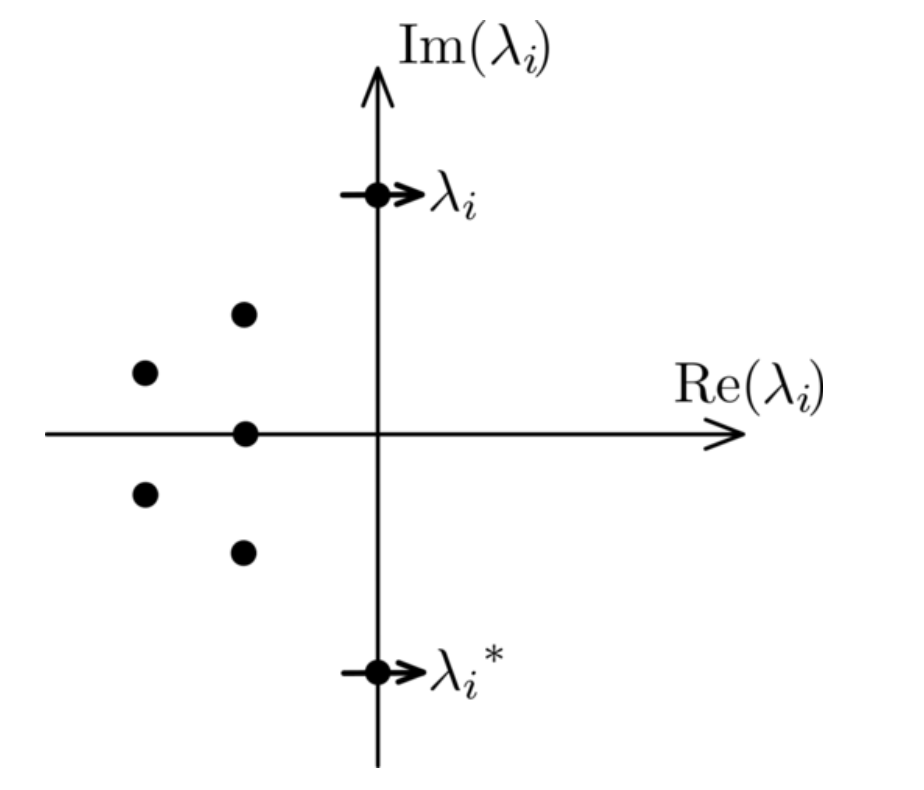
\includegraphics[width=13cm]{math_pics/hopf-bif-eigenvalue-graph.png}
	\centering
	\caption{Visualizing the zeroes}
\end{figure}

In $\mathbb{R}^2$, such Bifurcations cause special kinds of invariant sets, namely \textbf{limit cycles} to appear. These are periodic solutions, for which we'll need a few more concepts in order to be able to define them:
\begin{definition} \textbf{Closed trajectory and Closed orbit (cycle)}

	A trajectory (or flow): $y(t) \in \mathbb{R}^2$ as in Def. \ref{dyn_sys_orbit_flow_etc_def} is a solution for \ref{eq:1-d_bif_sys}

	A closed trajectory is one which returns to its starting point $\forall s_0 := \Phi(0,s) $ it has, namely:
	\begin{gather*}
		\exists t_0 \in T : \Phi(t,s) = \Phi(t+t_0,s), \forall s \in \Phi_{s_0}     \\
		\Updownarrow \\
		\exists t_0 \in T : y(t) = y(t+t_0), \forall t \in T
	\end{gather*}
	A \textbf{closed orbit} or \textbf{cycle} is just the image of such a closed trajectory.
\end{definition}

\begin{definition}\textbf{Limit point}
	These can be grouped into $\omega$ (attracting) and $\alpha$ (repelling) limit points:

	$y_\omega$ is an $\omega$-limit point  for $y$ if:

	$\exists (t_n)_{n \in \mathbb{N}} \subseteq I(y) : $
	\begin{gather*}
		\lim_{n \rightarrow \infty} t_n = \infty  \\
		\lim_{n \rightarrow \infty} \Phi(t_n,y) = y_\omega
	\end{gather*}
	And similarly, but in reverse:

	$y_\alpha$ is an $\alpha$-limit point  for $y$ if:

	$\exists (t_n)_{n \in \mathbb{N}} \subseteq I(y) : $
	\begin{gather*}
		\lim_{n \rightarrow \infty} t_n = \textbf{--} \infty  \\
		\lim_{n \rightarrow \infty} \Phi(t_n,y) = y_\alpha
	\end{gather*}
\end{definition}

\begin{definition}\textbf{Limit set}
	The set of all $\omega$ (or $\alpha$)-limit points for a particular orbit $\gamma$ is called the \textbf{limit set} of $\gamma$, denoted and defined as:
	\[
		\lim_{\omega}\gamma_s := \bigcap_{t \in T} \overline{ \{ \Phi(t', s) : t' > t \} }
	\]
	\[
		\lim_{\alpha}\gamma_s := \bigcap_{t \in T} \overline{ \{ \Phi(t', s) : t' < t \} }
	\]
\end{definition}

\begin{definition} \textbf{Limit cycle}

	A Limit Cycle is a cycle which is the limit set of at least another trajectory.
	Also, interestingly:
	\[
		\lim_{\omega}\gamma \bigcap \gamma  = \emptyset \implies \text{ it's an } \omega \text{-limit cycle}.
	\]
	\[
		\lim_{\alpha}\gamma \bigcap \gamma  = \emptyset \implies \text{ it's an } \alpha \text{-limit cycle}.
	\]
\end{definition}

//TODO: Proof: trust me bro;

What's interesting though, and makes calculations easier for the 2-D case is:
\begin{theorem}  \textbf{Poincaré-Bendixson}

	For a dynamical system $(T,X,\Phi)$ with $X \subseteq \mathbb{R}^2$, $\forall$ compact invariant set $S$:
	\begin{gather*}
		\text{if } \nexists x_0 \in S : \Phi(t_1, x_0) = \Phi(t_2,x_0), \forall t_1,t_2 \in T \\
		\Downarrow \\
		\forall s \in S: \gamma_s \text{ are either limit cycles, or } \lim_{\omega / \alpha}\gamma_s \text{ is an $\omega$ (or $\alpha$)-limit cycle }.
	\end{gather*}
\end{theorem}

But the problem is this theorem only holds for $\mathbb{R}^2$. For higher dimensions we don't have this property necessarily, instead we have to look for periodic solutions (limit cycles) ourselves - which, as stated previously - occur naturally during a Hopf bifurcation.

So having these in mind, Hopf is kind of like an $\mathbb{R}^n$ version of Pitchfork bif.: \ref{pitchfork_bif} when you think about it.

You can even see the resemblance in the way they look

\begin{figure}[H]
	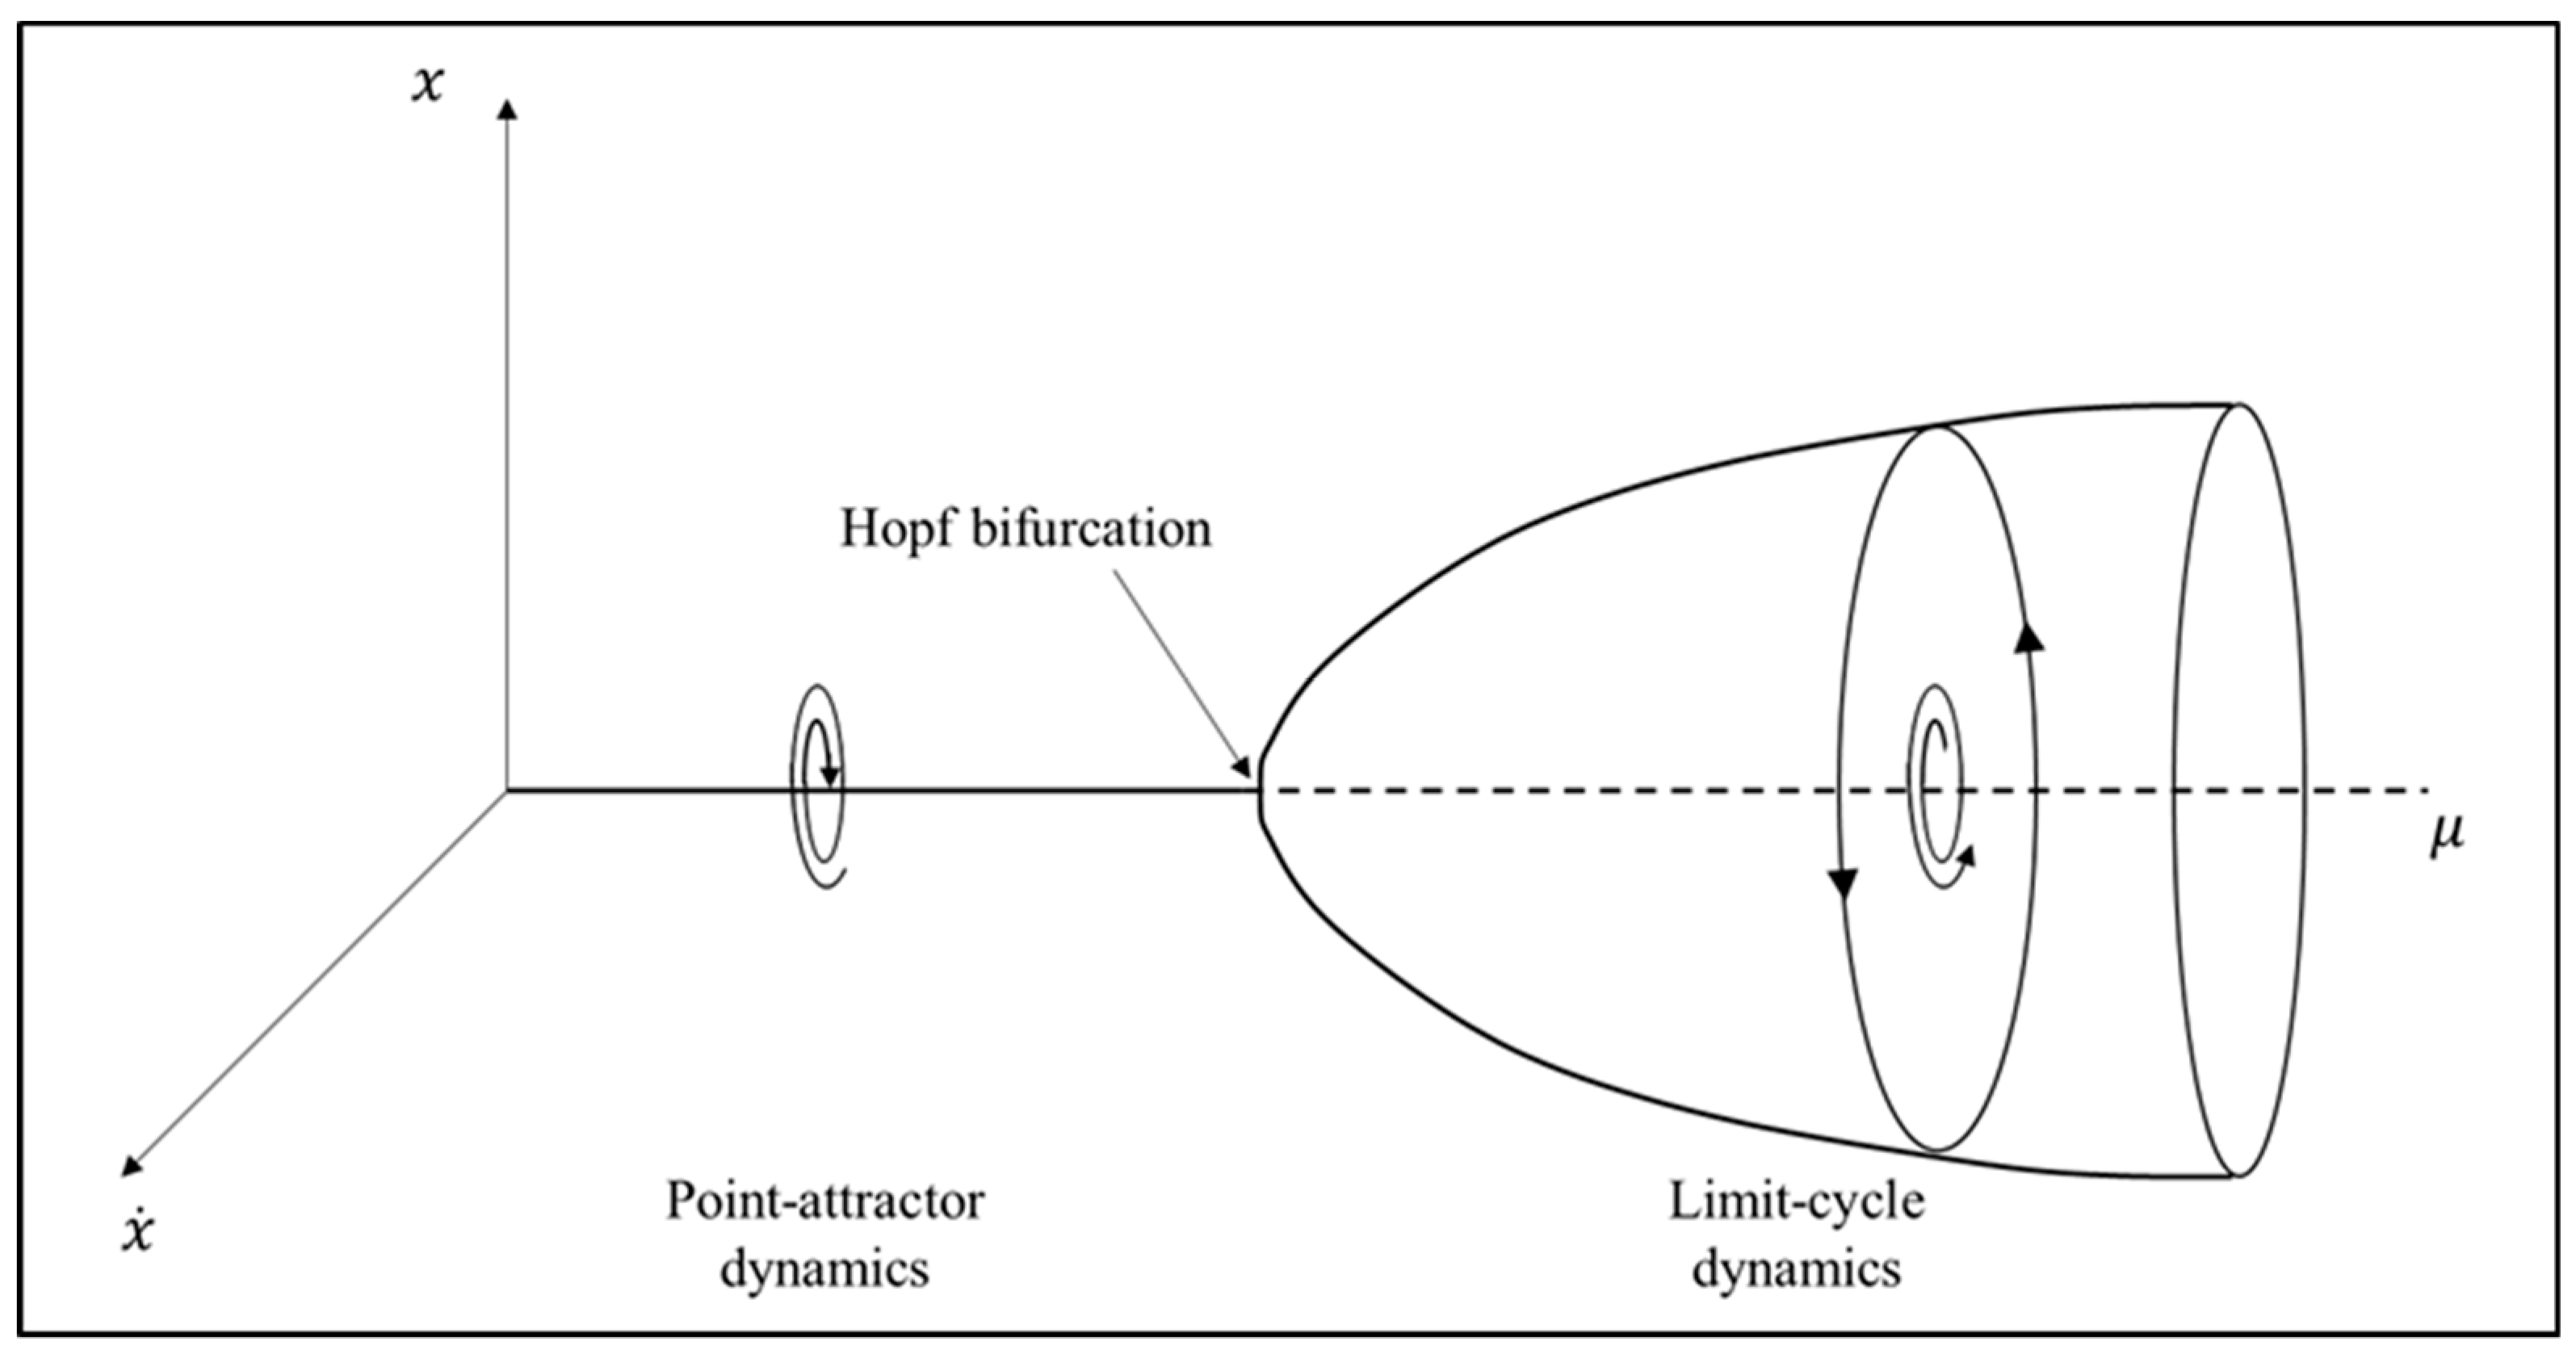
\includegraphics[width=13cm]{math_pics/hopf-bif-pic.png}
	\centering
\end{figure}


\includegraphics[width=11cm]{math_pics/leo.jpg}

\begin{figure}[H]
	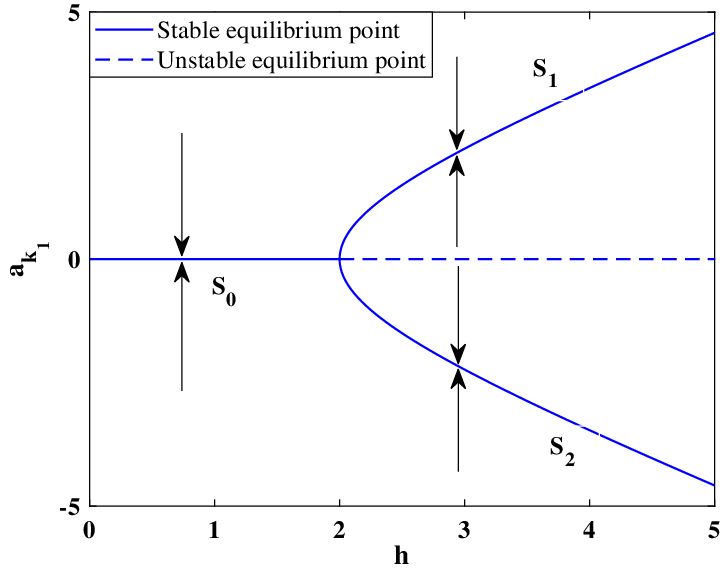
\includegraphics[width=13cm]{math_pics/pitchfork-photo.png}
	\centering
	\caption{Pitchfork bifurcation}
\end{figure}

\hfill\break
//TODO: scrie (si fa mai mult research) despre  \textbf{normal form} si despre cum aproximeaza el sistemul dinamic in jurul punctelor de bifurcatie, ca o sa-ti fie de folos la cam toate punctele de birufcatie sincer pare important si chiarn u stiu de el am vzt in mai multe parti

//TODO: sincer mai bine lasa tbh noone cares as of now
\hfill\break

\subsection{Proving the existence of simple Hopf bifurcations}

Finding necessary conditions for their existence makes use of a tool defined in the previous chapter (\ref{hurwitz_theorem}) the \textbf{Hurwitz matrix}.

Instead, now the characteristic polynomial depends on this new bifurcation parameter $\mu$.

\begin{proposition}\label{symmetric_roots_pair_criterion}
	Take $p_{\mu_0} \in \mathbb{C}^n[Z]$ with $n \geq 2$ and consider $\mu_0$ fixed:
	\[
		p_{\mu_0}(z) = a_0(\mu_0)z^n + a_1(\mu_0)z^{ n-1 } + \dots + a_n (\mu_0)
	\]

	Take $H_i(\mu_0)$ to be $p$'s $i$-th Hurwitz Matrix (\ref{hurwitz_theorem})

	If we have:
	\begin{gather*}
		\text{det }H_1(\mu_0) > 0 , \dots, \text{det }H_{n-2} (\mu_0) > 0. \\
		\Downarrow \\
		p_{\mu_0}(z) \text{ has } \leq 1 \text{ pair of symmetric roots  }
	\end{gather*}

	And $\exists!$ pair of symmetric roots $\iff \text{det}H_{n-1}(\mu_0) = 0$.

	If $a_n(\mu_0) > 0 \implies$ for the pair $\lambda_i, \overline{\lambda_i}$  : Re$(\lambda_i) =$ Re$(\overline{\lambda_i}) = 0$.
\end{proposition}

Now, more specifically, the necessary conditions for a simple Hopf bifurcation are:

\begin{proposition}\label{yangs_criterion}
	(Yang)
	A simple Hopf bifurcation occurs at fixed point $x^*$ and at the parameter threshold $\mu_0$ $\iff$
	\begin{gather*}
		\rom{1} \quad \text{det } H_{ n-1 }(\mu_0) = 0 \text{  and  } a_s(\mu_0) > 0, \\
		\rom{2} \quad 		\text{det }H_1(\mu_0) > 0 , \dots, \text{det }H_{n-2} (\mu_0) > 0 \text{  and  } \\
		\rom{3} \quad \left. \frac{d(\text{det }H_{n-1}(\mu))}{d\mu} \right|_{\mu = \mu_0} \neq 0.
	\end{gather*}
\end{proposition}

\subsection{Ruling out simple Hopf bifurcations}

Directly from criterion \ref{symmetric_roots_pair_criterion} we have a criterion for showing $\nexists \mu$ for which $x(\mu)$ undergoes simple Hopf bifurcations.
\begin{theorem}\label{ruling_out_simple_hopf_bif}

	For the dynamical system $\dot{x} = f_\mu(x)$ assume $\exists$ a curve of steady states $x(\mu)$.
	$p_\mu(z)$ is the characteristic polynomial of degree $s \geq 2$ of the linearization $J(x(\mu), \mu)$, and $H_i(\mu)$ its $i$-th Hurwitz matrix. Given:
	\[
		\text{det }H_1(\mu_0) > 0 , \dots, \text{det }H_{n-2} (\mu_0) > 0. \forall \mu
	\]
	And either:
	\begin{gather*}
		a_s(\mu) \leq 0 \text{whenever  det } H_{s-1} = 0  \\
		\text{or} \\
		\text{det }  H_{s-1}(\mu) \neq 0, \forall \mu    \\
		\Downarrow
	\end{gather*}
	$\nexists$ simple Hopf bifurcation $\forall \mu$ at the steady states $x(\mu)$.
\end{theorem}

\subsection{Convex parameters}\label{convex_paramteres}
With most dynamical systems, if we want to analyze their behavior we have to find, through all possible values if $\exists x^*(\mu)$ fixed points for which bifurcation occur, and hence we need to find any value $\exists \mu$ of the bifurcation parameter for which said bifurcation occurs, throughout our entire domain.

But luck would have it, though that the kind of systems we care about in this thesis, namely chemical reaction systems, defined in more detail in \ref{mass-action_network}, are not like "most" dynamical systems.

They all have a certain structure and their corresponding differential equations look in a way that can be represented more manageably.

Take now a system for a CRN, written as well in its matrix form, as in \ref{crn_system_matrix_form}
\[
	\dot{x} = f(k,x) :=\Gamma v(k,x)
\]
Where $v$, the flux vector, as in \ref{flux_vector} can be written as:
\[
	v(k, x) = \text{diag}(k)\Psi(x).
\]
as well.
Where diag $: \mathbb{C}^n \rightarrow \mathcal{M}_n(\mathbb{C})$,
\begin{align*}
	(\text{diag}(x))_{i,i} = x_i, \quad \forall i = \overline{1,n} \\
	(\text{diag}(x))_{i,j} = 0, \quad \forall i,j = \overline{1,n} , i \neq j.
\end{align*}
And $\Psi(x)$ is the flux vector, where the reaction rates \ref{reaction_rate} are written without the leading $k_i$'s, only depending on $x$.

If we want to look into how the system behaves near equilibrium points $x^*$ we have to, just like other systems, study their Jacobian matrix, which, because the flux vector is made of polynomials can be written using this little trick:
\[
	J(k, x)_{\mid x=x^*}=\Gamma \operatorname{diag}\left(v\left(k, x^*\right)\right) \Gamma_L^T \operatorname{diag}\left(\frac{1}{x^*}\right)
\]

Now since $x^*$ is a fixed point, the flux vector satisfies:
\begin{equation}\label{flux_vector_linear_problem}
	\Gamma v(k,x^*) = 0, \quad v \geq 0.
\end{equation}
And so the solutions of (\ref{flux_vector_linear_problem}) are a \textbf{convex polyhedral cone} called the \textbf{flux cone}.

A flux cone is expressed as an $\mathbb{R}_{\geq 0}$ linear combination of it extreme vectors $\left\{ E_1 , \ldots , E_l \right\}$.

\begin{definition}\label{convex_params_definition}
	\textbf{Convex parameters.}
	\begin{equation}\label{flux_cone}
		\boxed{		v=\sum_{i=1}^l \lambda_i E_i=E \lambda, \quad \lambda_i \geq 0, \forall i = \overline{1,l} }
	\end{equation}
	Where $\lambda_i$ are called \textbf{convex parameters}.
\end{definition}
But we also need something to parametrize the $x$'s, so:
\begin{equation}\label{other_convex_parameters}
	\boxed{	h_i=\frac{1}{x_i^*}, \quad i = \overline{1,n} }
\end{equation}
So having this in mind:
\begin{definition}
	A convex parameter vector:
	\[
		(h, \lambda) = (h_1, \ldots, h_n , \lambda_1, \ldots , \lambda_l) \in \mathbb{R}_{>0}^n \times \mathbb{R}_{\geq 0}^{l} : E \lambda \in \mathbb{R}^r_{> 0}.
	\]
	With $E$ the matrix whose columns are the convex polyhedral cone's extreme vectors.
\end{definition}
So we may write the Jacobian using this new coordinate system, which in turn makes its coefficients monomials, instead of the usual polynomial and multiple-term expressions you usually get with these systems, like in Ex. (\ref{bigger_network_example1}).
\newcommand\eqCuzConvex{\stackrel{\mathclap{\normalfont\mbox{\ref{flux_vector_linear_problem}, \ref{convex_params_definition}}}}{=\joinrel=\joinrel=\joinrel=\joinrel=}}

\begin{gather}\label{jacobian_convex_params}
	v(k, x^*) \eqCuzConvex E \lambda  \notag \\
	\Downarrow \text{ \ref{other_convex_parameters} } \notag \\
	\boxed{J(k,x)_{|x=x^{*}}=J(h,\lambda)=\Gamma \text{diag}(E\lambda)\Gamma_{L}^{T}\text{diag}(h)}
\end{gather}

We could, of course turn this convex vector back into the regular coordinate system:

Given:
\begin{gather*}
	(h,\lambda) \Downarrow \\
	\text{Let  } x^* \in \mathbb{R}^n , \boxed{
		x^*_i = \frac{1}{h_i} , i = \overline{1,n}
	} \\
	\boxed{
		k = \text{diag}(\Psi(h)) E \lambda \in \mathbb{R}^r_{> 0}
 }
\end{gather*}

\hfill\break
//TODO: Aici trebuie re-introducere la notatia specifica pt reactiile chimice, si adica mai bine te pui sa vb despre asta in primele capitole de "Introduction to chemical reaction networks"
si asta o sa fie pt orice fel de reactii chimice, nu doar pt astea de mai jos:
Poti sa te folosesti nu numa de prezentare da si din lucrarea lui conradi ca zice chestii mai specifice asa sa zic nuj.

//TODO sa mai zici si tu cand e si cand te intereseaza ce e ala flux cone si cum functioneste
\hfill\break

\section{What is a Phosphorylation-Dephosphorylation CRN?}

\hfill\break
//TODO: Povestesti frumos specific pt asta ce sunt, din nou, te iei din ce s-a vb in prezentare da poate un pic si din ala alu conradi
\hfill\break

Phosphorylation of proteins occurs in cycles, which are fueled by $3$ proteins which are the ingredients: A substrate $S$ and $2$ enzymes: kinase ($K$) and phosphatase ($F$).

The one that starts this chain is the kinase ($K$), attaching phosphate groups onto the substrate, phosphorylating it.

Then, phosphatase ($F$) comes in and undoes all the hard work kinase ($K$) put in and removes the phosphate groups, now dephosphorylating the substrate.

\hfill\break
These cycles are a particular case of a broader type of what are called \textbf{posttranslational modification (PTM) systems.} Another example would be, for instance \textbf{methylation}.

The reason we care about them is their key implication in \textbf{ signal transduction}, which is the process our cells use to communicate with one-another. Any disturbance in this system is linked to its own class of health complications in our body.

Basically, do these biochemical systems induce periodic solutions as in (\ref{hopf_bif_def}), likening clocks, or do they have multiple steady-states (\textbf{capacity for bistability}), likening switches?

What these all have in common, though are the \textbf{building blocks} used to create them:
\begin{equation}\label{ptm_building_blocks}
	S+M \xrightleftharpoons[k_2]{k_1} SM \xrightarrow{k_3} S^* + M \quad \mathrm{~and~} \quad S^* + U \xrightleftharpoons[k_5]{k_4} S^* U \xrightarrow{k_6} S + U
\end{equation}

What's familiar to the previous example is the presence of a substrate ($S$), which forms the \textbf{complex} ($SM$) with the \textbf{modifier} ($M$), which - as the name implies - modifies ($S$) to become ($S^*$), which then dissociates with ($M$);

And just like in dephosphorylation, another modifier ($U$) can come in and undo the entire hustle ($M$) did.

So the \textbf{phosphorylation version of this would be}:
\begin{gather*}\label{phosphorylation_reaction_basis}
	S_0 + K \xrightleftharpoons[k_2]{k_1} K S_0 \xrightarrow{k_3} S_1 + K  \xrightleftharpoons[k_5]{k_4} \ldots K S_{n-1} \xrightarrow{k_{ 3n}} S_n + K  \\
	\text{ for the phosphorylation side, and} \\
	S_n + F \xrightleftharpoons[k_{2(n+1)}]{k_{2n+1}} F S_n \xrightarrow{k_{2n + 3}} S_{n-1} + F  \xrightleftharpoons[k_{2n + 5}]{k_{2n + 4}} \ldots F S_{1} \xrightarrow{k_{6n}} S_0 + F  \\
	\text{ for the dephosphorylation side, and}
\end{gather*}
Which phosphorylates the substrate ($S$) up to a certain number of phosphate groups $n$, and then \textbf{de}phosphorylates it back to 0, where the subscript notation $S_i ;  i = \overline{1,n}$ represents the substrate ($S$) with its $i$ phosphate groups.

\subsection{Cyclic and mixed distributive and processive Phosphorylation-Dephosphorylation CRN}
The system above represents a \textbf{distributive} cycle, meaning each bounding site of ($K$) and ($F$) (de)phosphorylate only one single phosphate group.

As opposed to a \textbf{processive} one, which would look something like:
\begin{equation*}
	S_0 + K \xrightleftharpoons[k_2]{k_1} S_0 K \xrightarrow{k_3} S_1 K \xrightarrow{k_4} S_2 + K
\end{equation*}
For a binding one, and
\begin{equation*}
	S_2 + F \xrightleftharpoons[k_2]{k_1} S_2 F \xrightarrow{k_3} S_1 F \xrightarrow{k_4} S_0 + F
\end{equation*}
For the unbinding operation.

Notice the following reactions where the enzymes don't dissociate.
\begin{gather*}
	\ldots S_0 K \xrightarrow{k_3} S_1 K \xrightarrow{k_4} \ldots \\
	\ldots S_2 F \xrightarrow{k_3} S_1 F \xrightarrow{k_4} \ldots	
\end{gather*}

It was shown that processive systems are globally stable and distributive ones may be bistable (having multiple steady states).

There are also extra classifications in double phosphorylation systems:

The order phosphorylation occurs matters too, so if:
\rom{1}: If the \text{last} phosphorylated site is being dephosphorylated in the first dephosphorylation binding, then the mechanism is said to be \textbf{sequential}.

\rom{2} Whereas, if the \text{first} phosphorylated site is being \textbf{de}phosphorylated first then the system is \textbf{cyclic}.

You can see here an example of this classification in two mechanisms that, while they differ in this category, they are still both distributive.
\begin{figure}[H]
	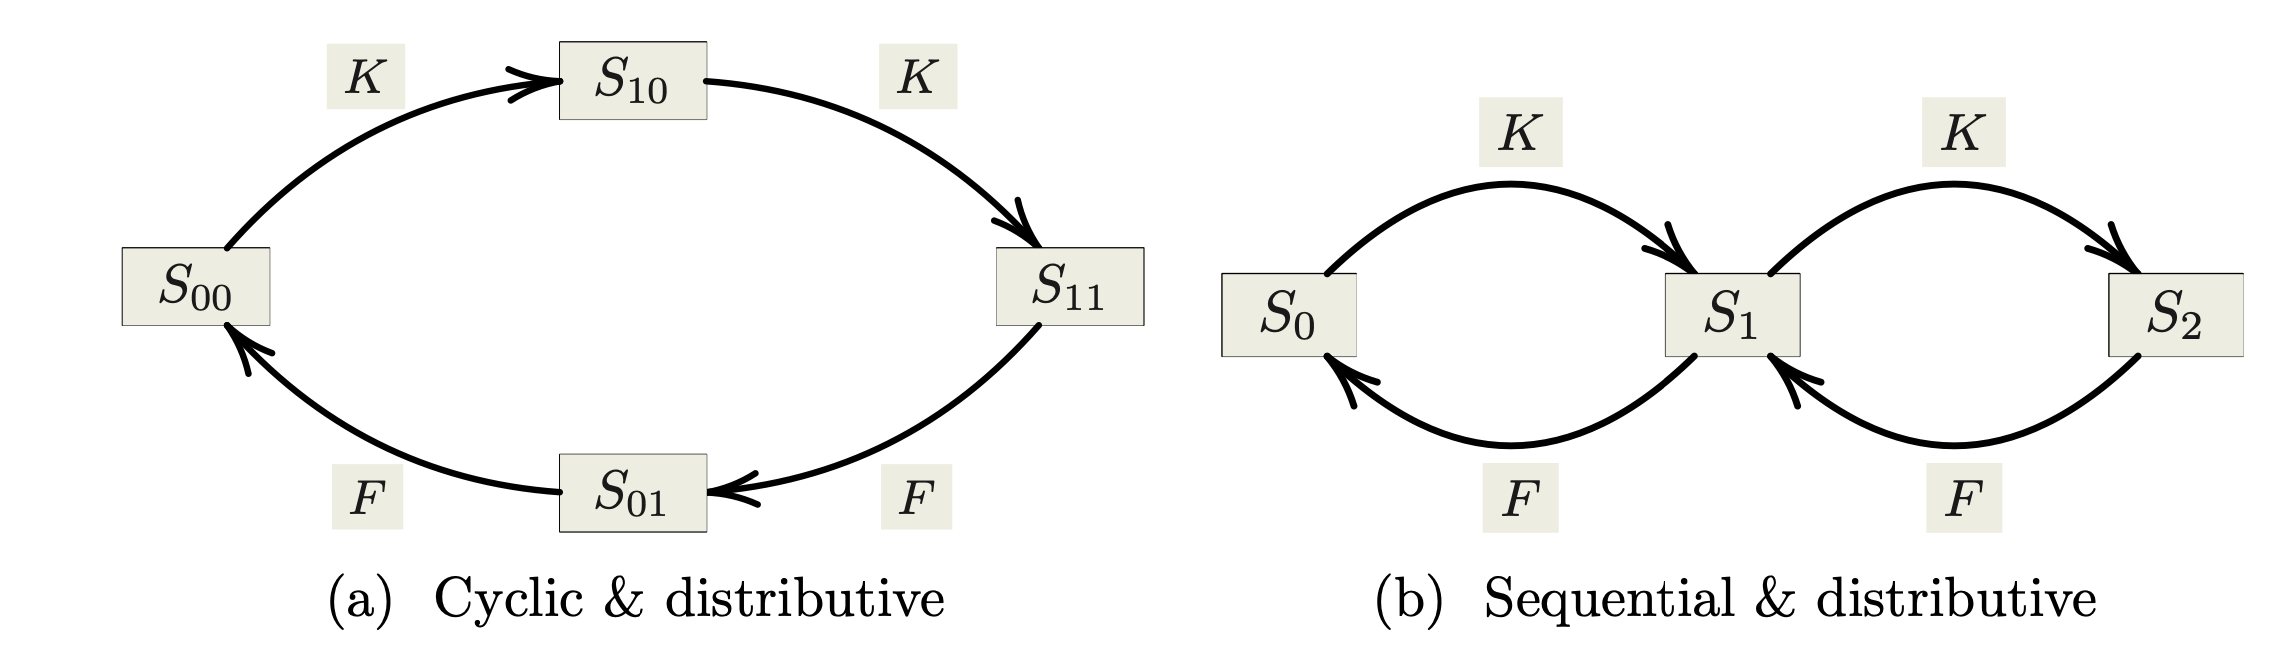
\includegraphics[width=13cm]{math_pics/cyclic-vs-sequential.png}
	\centering
\end{figure}
In the left one here, $S_{ij}$ shows which one of the $2$ binding sites gets phosphate groups attached to it, (Ex, $S_{10}$: first one is phosphorylated, second not).

\hfill\break
//TODO: de ce ne intereseaza specfic phospho, de phosho?
\hfill\break

\hfill\break
//TODO: 1. scrii despre un exemplu care arata cand nu se gases bifuractii
\hfill\break

We'll now try to solve the problem whether a particular system undergoes simple Hopf bifurcations.

Take, for example, the following basic cycle:
\textbf{Example 1}:
\begin{figure*}[h]
	\text{\\TODO: cum drq desenez si eu frumusel cu sageti in latex sa fac asa la toate:}
	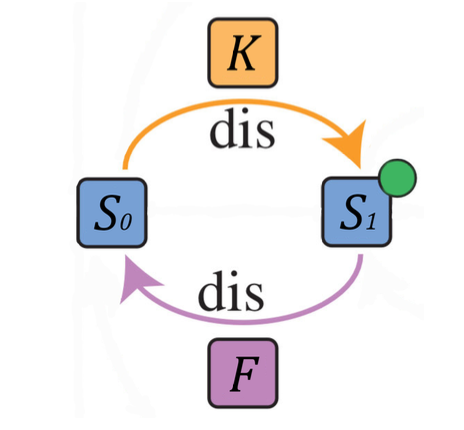
\includegraphics[width=38mm]{math_pics/ex1-no-bifurcations.png}	
	\centering
\end{figure*}

Whose chemical reaction notation looks like:
\begin{gather}\label{network1}
	K + S_0 \xrightleftharpoons[k_2]{k_1} K S_0 \xrightarrow{k_3} K + S_1 \tag{$\mathcal{N}_1$} \\
	F + S_1 \xrightleftharpoons[k_4]{k_5} F S_1 \xrightarrow{k_6} F + S_0 \notag
\end{gather}

\textbf{Remark 1:} $(a)$ As you can see, the network (\ref{network1}) consists of $6$ species ($2$ substrates $S_0$, $S_1$; $2$ enzymes $K$, $F$; which together form $2$ complexes: $K S_0$, $F S_1$) and $6$ reactions ($2$ reversible and $2$ irreversible) with matrix subspace $=$ rank $\Gamma = 3$.

Using \href{https://github.com/viktorashi/Open-CoNtRol}{the app} I've generated the following stoichiometric matrices, its rank and its corresponding dynamical system:

\begin{align*}
	\Gamma &=
	\begin{pmatrix}
		K & -1 &  1 &  1 &  0 &  0 &  0 \\
		S0& -1 &  1 &  0 &  0 &  0 &  1 \\
		KS0 &  1& -1& -1 &  0 &  0 &  0 \\
		S1 &  0 &  0 &  1& -1 &  1 &  0 \\
		F &  0 &  0 &  0& -1 &  1 &  1 \\
		FS1 &  0 &  0 &  0 &  1& -1& -1  \\		
	\end{pmatrix}, \quad \text{rank}(\Gamma) = 3 \\[3ex]
	\Gamma_L &=
	\begin{bmatrix}
		1&0&0&0&0&0\\
		1&0&0&0&0&0\\
		0&1&1&0&0&0\\
		0&0&0&1&0&0\\
		0&0&0&1&0&0\\
		0&0&0&0&1&1
	\end{bmatrix} \\[3ex]
	&
	\begin{cases*}
		\begin{array}{ll}
			\dot{x}_1(t) = -k_4 x_1(t) *x_6(t)+k_5 x_2(t)+k_6 x_2(t) \\
			\dot{x}_2(t) = k_4 x_1(t) *x_6(t)-k_5 x_2(t)-k_6 x_2(t) \\
			\dot{x}_3(t) = -k_1 x_3(t) *x_5(t)+k_2 x_4(t)+k_3 x_4(t) \\
			\dot{x}_4(t) = k_1 x_3(t) *x_5(t)-k_2 x_4(t)-k_3 x_4(t) \\
			\dot{x}_5(t) = -k_1 x_3(t) *x_5(t)+k_2 x_4(t)+k_6 x_2(t) \\
			\dot{x}_6(t) = k_3 x_4(t)-k_4 x_1(t) *x_6(t)+k_5 x_2(t) \\
		\end{array}	
	\end{cases*}
\end{align*}
Where the "species to index mapping" is:
\[
	F:  x_1
 | FS1: x_2
 | K: x_3
 | KS0: x_4
 | S0: x_5
 | S1: x_6
\]
\textbf{Remark 1:} $(b)$ For the network (\ref{network1}), the cone (defined as in \ref{flux_cone}) $\Gamma v(k,x) = 0, \forall v \geqq 0$ is spanned by the vectors $w_0, w_1, w_2 \geqq 0 : \lambda_0 w_0 + \lambda_1 w_1 + \lambda_2 w_2 \geqq 0 \iff \lambda_1, \lambda_2, \lambda_3 \geq 0$.

Now we may consider the Jacobian written in convex parameters for network (\ref{network1}), $J_1(h,\lambda)$ as defined in \ref{jacobian_convex_params}, which is parametrized by $9$ parameters: $\lambda_0, \lambda_1, \lambda_2$ and $h_1, \ldots, h_6$.

So, from \textbf{Remark 1} $(a)$ and $(b)$, it follows that the characteristic polynomial of $J_1(h, \lambda)$ is
\[
	p_{h,\lambda}(z) = z^3 (a_0(h,\lambda) z^3 + a_1(h, \lambda)z^2 + a_2 (h,\lambda)z + a_3(h,\lambda) )
\]
Where each coefficient $a_i, i = \overline{0,3}$ depends on these $9$ parameters.

Now, with the motivation of (\ref{ruling_out_simple_hopf_bif}) in mind, we compute the values of $a_i(h,\lambda), i = \overline{0,3}$ and det$H_i(h,\lambda), i = \overline{1,2}$ according to (\ref{hurwitz_theorem}), obtaining the following proposition:
\begin{proposition}
	Based on the notation above, for the network (\ref{network1}):

	det$H_1(h,\lambda)$, det$H_2(h,\lambda)$ and $a_3(h,\lambda)$ contain only positive monomials. Thus, det$H_1(h,\lambda)$, det$H_2(h,\lambda) \geq 0, \forall h, \lambda \geqq 0$, specifically det$H_2(h,\lambda) \neq 0$, $\lightning$ (\ref{ruling_out_simple_hopf_bif}).
\end{proposition}
\begin{proof}
	Given the network structure defined above, as well as the $E\lambda$ matrix made of the extreme cone vectors (\textbf{ray}):
	\[
		E\lambda =
		\begin{bmatrix}
			\lambda_2 + \lambda_3 \\
			\lambda_1 \\
			\lambda_3 \\
			\lambda_2 + \lambda_3 \\
			\lambda_2 \\
			\lambda_3
		\end{bmatrix}
	\]
	The Jacobian in convex parameters, as given in (\ref{jacobian_convex_params}), using the Maple script is:
	\[
		J_1(h,\lambda)=
		\text{//TODO: si acm te pui tu sa rulezi scriptu de maple in virtual machinu ala}
	\]
	Then by means of another Maple script, we can write the Hurwitz matrices of its corresponding characteristic polynomial.
	\[
		\text{//TODO: doar pune aici ce iti da maplru}
	\]
	Just by looking at $H_2(h,\lambda)$, we can deduce that $a_{ij}$ is a positive monomial, for all  its entries $\forall h , \lambda > 0$, in particular det$H_2(h, \lambda) \neq 0$.

	So, det$H_1(k,x^*) > 0, \forall k, x^* > 0$, moreover the coefficient of the largest degree term in the characteristic polynomial $a_3(k, x^*) > 0$, so according to \ref{ruling_out_simple_hopf_bif} : For network (\ref{network1}), $\nexists k, x^* \geqq 0$ for which $J_1(k,x^*)$ has a pair of purely imaginary eigenvalues $\implies \nexists$ a simple Hopf bifurcation in our system for any rate constants or positive steady states
\end{proof}

\newpage
\textbf{Example 2}:
Now let us apply the same method and intuition for the following network.
\begin{figure}[H]
	\text{\\TODO: cum drq desenez si eu frumusel cu sageti in latex sa fac asa la toate:}
	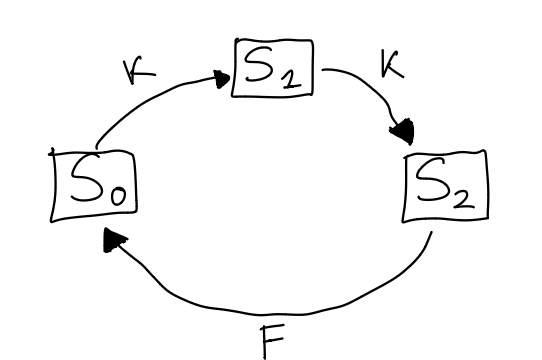
\includegraphics[width=13cm]{math_pics/ex2-no-bifurcations.png}
	\centering
\end{figure}
Its chemical reaction network is:
\begin{align*}
	S_0+K &\xrightleftharpoons[k_2]{k_1} KS_0 \xrightarrow{k_3} S_1 + K \xrightleftharpoons[k_5]{k_4} KS_1 \xrightarrow{k_6} S_2 + K \\
	S_2+F &\xrightleftharpoons[k_8]{k_7} FS_2 \xrightarrow{k_9} S_0 + F
\end{align*}
\textbf{Remark 2:} $(a)$ Here the system is composed of $8$ species: The two enzymes like before, $K$ and $F$, but $K$ not phosphorylates up to $S_2$ and hence forms the complexes $KS_0$, $KS_1$ as well, so as a consequence, now $F$ \textbf{de}-phosphorylates starting from $FS_2$, and because the network is cyclic, it skips directly to the disassociated relation $S_0 + F$.

We also now have $9$ reactions: $3$ reversible, $3$ irreversible.

Now the app generated the following:
\begin{align*}
	\Gamma &=
	\begin{pmatrix}
		S0& -1&\ 1&\ 0&\ 0&\ 0&\ 0&\ 0&\ 0&\ 1\cr K& -1&\ 1&\ 1& -1&\ 1&\ 1&\ 0&\ 0&\ 0\cr KS0&\ 1& -1& -1&\ 0&\ 0&\ 0&\ 0&\ 0&\ 0\cr S1&\ 0&\ 0&\ 1& -1&\ 1&\ 0&\ 0&\ 0&\ 0\cr KS1&\ 0&\ 0&\ 0&\ 1& -1& -1&\ 0&\ 0&\ 0\cr S2&\ 0&\ 0&\ 0&\ 0&\ 0&\ 1& -1&\ 1&\ 0\cr F&\ 0&\ 0&\ 0&\ 0&\ 0&\ 0& -1&\ 1&\ 1\cr FS2&\ 0&\ 0&\ 0&\ 0&\ 0&\ 0&\ 1& -1& -1\cr
	\end{pmatrix}, \quad \text{rank}(\Gamma) = 5 \\[3ex]
	\Gamma_L &=
	\begin{bmatrix}
		1 & 0 & 0& 0& 0& 0& 0& 0& 0 \\
		1 & 0 & 0& 1& 0& 0& 0& 0& 0 \\
		0 & 1 & 1& 0& 0& 0& 0& 0& 0 \\
		0 & 0 & 0& 1& 0& 0& 0& 0& 0 \\
		0 & 0 & 0& 0& 1& 1& 0& 0& 0 \\
		0 & 0 & 0& 0& 0& 0& 1& 0& 0 \\
		0 & 0 & 0& 0& 0& 0& 1& 0& 0 \\
		0 & 0 & 0& 0& 0& 0& 0& 1& 1 \\
	\end{bmatrix}, \quad \text{rank}(\Gamma_L) = 8 \\[3ex]
	&
	\begin{cases*}
		\begin{array}{ll}
			\dot{x}_1(t) = -k_7 x_8(t) *x_1(t)+k_8 x_2(t)+k_9 x_2(t) \\
			\dot{x}_2(t) = k_7 x_8(t) *x_1(t)-k_8 x_2(t)-k_9 x_2(t) \\
			\dot{x}_3(t) = -k_1 x_6(t) *x_3(t)+k_2 x_4(t)+k_3 x_4(t)-k_4 x_7(t) *x_3(t)+k_5 x_5(t)+k_6 x_5(t) \\
			\dot{x}_4(t) = k_1 x_6(t) *x_3(t)-k_2 x_4(t)-k_3 x_4(t) \\
			\dot{x}_5(t) = k_4 x_7(t) *x_3(t)-k_5 x_5(t)-k_6 x_5(t) \\
			\dot{x}_6(t) = -k_1 x_6(t) *x_3(t)+k_2 x_4(t)+k_9 x_2(t) \\
			\dot{x}_7(t) = k_3 x_4(t)-k_4 x_7(t) *x_3(t)+k_5 x_5(t) \\
			\dot{x}_8(t) = k_6 x_5(t)-k_7 x_8(t) *x_1(t)+k_8 x_2(t) \\
		\end{array}	
	\end{cases*}
\end{align*}

\hfill\break

\hfill\break
//TODO: 3. de cum s-a folosit pt un network de s-ai eliminat cate 2 specii si s-a facut tabel cu diverse sisteme care sunt mostenite din el
deci practic un ucare chiar a gasit bifurcatii, toata nebunia aia de s-a scris despre ea de cum au reusit sa demonstreze ca chiar exista bifurcatii si sa le si gaseasca valorile pt care sunt
\hfill\break
